% !TEX encoding = UTF-8 Unicode

\documentclass{article}

\usepackage{a4wide}
\usepackage[utf8]{inputenc}
\usepackage[T1]{fontenc}
\usepackage[french]{babel}
\usepackage[babel=true]{csquotes} % guillemets français
\usepackage{graphicx}
\graphicspath{{Images/}}
\usepackage{color}
\usepackage{hyperref}
\hypersetup{colorlinks,linkcolor=,urlcolor=blue}

\usepackage{amsmath}
\usepackage{amssymb}


\title{Compte Rendu : DM sur les Threads}
\author{\'Kévin HOARAU, L3 informatique}
\date{\today}

\begin{document}

\maketitle % pour écrire le titre


%% Le résumé:
\begin{abstract}
  Dans ce rapport , je vais vous montrer comment créer un thread , la création d'une interface graphique (tKinter ou Swing) en python et Java et les difficultés rencontrées au cours des exercices 2.3 et 3.2.
\end{abstract}

\section{Introduction}
\label{section:hello} % pour faire référence à  la section ailleurs (\ref{...} voir plus bas)

Un processus est un programme ( fichier exécutable ) en cours d'exécution sur un processeur.
Il est caractérisé par :
\begin{itemize}
\item Son code
\item Son espace d'adressage
\item Son identifiant
\item Sa priorité 
\end{itemize}
Dans chaque processus, Il y a  des threads. Il est créé lorsqu'un autre processus lance son exécution. Un processus dispose d’un thread principal depuis lequel on peut lancés d’autres threads parallèlement(thread démon).
Lorsqu'on en crée plusieurs, on peut exécuter des tâches simultanément.Il est préférable de séparer les tâches dans plusieurs threads pour optimiser le programme.


En premier lieu, nous allons voir la notion de Thread. En deuxième lieu, nous parlerons d'interface graphique et puis nous finirons par voir ces notions et les difficultés rencontrées dans les exercices 2.3 et 3.2.

 
\section{Thread}
\subsection{Qu'est ce que c'est?}

Un Thread est un \textbf {fil d'exécution} de code à l'intérieur d'un processus et qui a la possibilité d'être ordonnancé (c'est un \textbf {"sous-processus"}).
	Les threads d'un même processus partagent le \textbf{même espace d'adressage}, le \textbf{même segment de code} et le \textbf{même segment de données} mais possèdent chacun leur \textbf{propre compteur de programme} et \textbf{ propre pile d'exécution}
 

% \cite{...} permet de faire référence à  des éléments de la
% bibliographie.

\subsection{Python}
En Python, pour créer et gérer des threads on utilise le module threading qui fournit la classe Thread.

Pour créer un thread, il suffit de surcharger la méthode \verb|run| de la classe Thread. Si le thread a besoin de données lors de son exécution, il faut surcharger son constructeur sans oublier d’appeler le constructeur de la classe mère. L’exécution de thread commence par la création d’une instance et l’appel à la méthode \verb|start|. En résumé, il faut retenir les éléments suivants :
\begin{itemize}
\item surcharger la classe \verb|threading.Thread|,
\item surcharger le constructeur sans oublier d’appeler le constructeur \verb|threading.Thread.__init__|
\item surcharger la méthode \verb|run|, c’est le code que devra exécuter le thread,
\item créer une instance de la nouvelle classe et appeler la méthode \verb|start| pour lancer le thread secondaire qui formera le second fil d’exécution.
\end{itemize}

\bigskip Code:

\begin{verbatim}
class ThreadProducteur(Thread):
    def __init__(self,texte, q, tempsSommeil, nom):
        Thread.__init__(self)
        self.texte = Label(fen, text="Thread Producteur : Ajout de l'entier .")
        self.texte.pack()
        self.message = texte
        self.q = q
        self.n=0
        self.tempsSommeil = tempsSommeil
        self.name = nom
        self.daemon = True

    def run(self):
        while True:
            self.ajout = randint(1,100)
            self.q.put(self.ajout, block=True,timeout=None)
            self.texte["text"] = "Thread Producteur : Ajout de l'entier {} .".format(self.ajout)
            self.ajout=0
            self.texte.pack(expand=True, timeout=None)
            time.sleep(self.tempsSommeil)
            
  p = ThreadProducteur(texte,q, 1, "p")
  p.start()
\end{verbatim}




\subsection{Java}

En Java, on va utiliser la classe \verb|Thread| qui se trouve dans le package \verb|java.lang|.
Pour créer un thread et donc avoir la tâche exécutée en parallèle, il faut appeler la méthode \verb|start| de la classe \verb|Thread|. Cette méthode fait deux choses : elle crée tout d'abord un nouveau thread d'exécution et elle y exécute ensuite la méthode \verb|run|.





Tout programme Java comporte au moins un thread principal correspondant a la methode main. 
Ci dessous ,on a le code courant du thread de la classe Main.

\begin{verbatim}
public class Main {
   public static void main(String[] args) {
      System.out.println("Hello World!");
   }
}
\end{verbatim}
Ce code affiche tout simplement un message : Hello World!

\section{Interface Graphique }

% \ref{...} permet de faire référence à  un élément défini
% ailleurs dans le document (voir \label{...} plus haut).
Une interface graphique (GUI: Graphical User Interface) ou un environnement graphique est un dispositif de dialogue homme-machine

\subsection{Python}

Pour créer une interface graphique en python, on utilise la bibliothèque \verb|Tkinter|.
\verb|Tkinter| a été renommé \verb|tkinter| en python 3.

\bigskip Voici un exemple de code en python:
\begin{verbatim} 
from tkinter import *

fenetre = Tk()
fenetre.title('File d’entiers')
fenetre.mainloop()
\end{verbatim}

\begin{center} \fbox{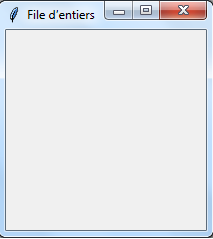
\includegraphics[scale=0.5]{Images/fenetrePython}}\end{center}

\subsection{Java}

Pour créer une interface graphique en Java, on utilise différentes bibliothèques mais essentiellement les packages \verb|javax.swing, java.awt|.

\bigskip Voici un exemple de code en Java:
\begin{verbatim} 
import javax.swing.*;

public class Fenetre extends JFrame {
	public Fenetre() {
      super("Balle en mouvement");
      setSize(350, 350);
      setLocationRelativeTo(null);
      setDefaultCloseOperation(EXIT_ON_CLOSE);
      setVisible(true);
   }
	public static void main(String[] args) { new Fenetre(); }	
}

 \end{verbatim} 
\begin{center}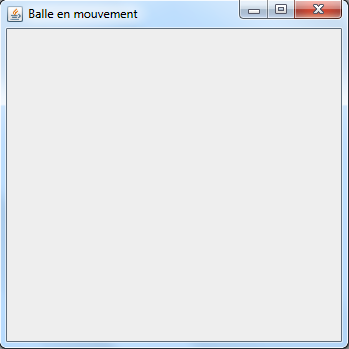
\includegraphics[scale=0.5]{Images/fenetreJava.png}\end{center}

\section{Difficultés rencontrées}
Maintenant je vais parlé des difficultés rencontrées au cours des exercices 2.3 et 3.2.
\subsection{Exercice 2.3}
Pour cette exercice, j'ai décidé de le faire sous Python. Au début, le problème que j'ai eu c'était qu'on devait appuyer sur la touche \textbf{Return} pour que les threads s'arrête.
J'avais essayé avec \textbf{input()} mais ça lancé le thread producteur après je devais cliquer sur \textbf{Return} pour lancer le thread Consommateur.
Pour résoudre ce problème j'ai utilisé un événement de clavier qui détecte les touches pressés du clavier.

\bigskip Voici le code que j'ai utilisé:
\begin{verbatim} 
def Clavier(event):
    touche = event.keysym
    if touche == 'Return':
        fen.destroy()
 \end{verbatim}

\subsection{Exercice 3.2}
Pour cette exercice, j'ai décidé de le faire sous Java. Il fallait faire une fenêtre avec des balles en mouvements dedans. En ajoutant des collisions, l'affichage du score et de l'horloge.
Je n'est pas pu finir cet exercice, il me manque les collisions, l'affichage du score et de l'horloge. Mais aussi la balle n'apparait pas(mais le tout dans un seul fichier ça fonctionne) et quelques détails dans le programme à régler(pause, quand on ajoute une balle c'est tjrs à la même position  etc).
%%% La bibliographie:
\bibliographystyle{plain}
\bibliography{ma_biblio}
\begin{thebibliography}{9}
\bibitem{wiki}
         Wikipedia : \url {https://fr.wikipedia.org/wiki/Interface_graphique}
 \bibitem{eve}       
         Notion d'évènement : \url {http://tkinter.fdex.eu/doc/event.html}
\bibitem{opcl}
	Thread, Fenetre, GUI : \url{http://openclassrooms.com/}
\end{thebibliography}
\end{document}
